\documentclass[tikz,border=8pt]{standalone}
\begin{document}
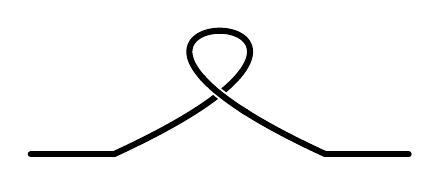
\begin{tikzpicture}[line cap=round,line join=round]
  \tikzset{strand/.style={draw=black,line width=2.2pt,fill=none}}
  % A rotated nodal cubic gives one smooth strand with one loop.
  \draw[strand] (-2.4,-0.77) -- (-1.344,-0.77);
  \draw[strand] plot[domain=-1.4:1.4,samples=180,smooth,variable=\t]
    ({\t*\t*\t-\t},{0.8*(1-\t*\t)});
  \draw[strand] (1.344,-0.77) -- (2.4,-0.77);
  % Redraw one branch at the double point to show which strand is above.
  \draw[white,line width=3.6pt] plot[domain=0.9:1.1,samples=24,smooth,variable=\t]
    ({\t*\t*\t-\t},{0.8*(1-\t*\t)});
  \draw[strand] plot[domain=0.86:1.14,samples=30,smooth,variable=\t]
    ({\t*\t*\t-\t},{0.8*(1-\t*\t)});
\end{tikzpicture}
\end{document}
